\documentclass{beamer}
\usepackage{graphicx}
\usepackage{verbatim}
\usepackage{xcolor}
\usepackage{colortbl}

\renewcommand{\figurename}{Gambar}
\renewcommand{\tablename}{Tabel}

\usetheme{metropolis}
\setbeamertemplate{navigation symbols}{}
\usepackage{listings}
\usepackage{xcolor}
\usepackage{ragged2e}

\definecolor{codegreen}{rgb}{0,0.6,0}
\definecolor{codegray}{rgb}{0.5,0.5,0.5}
\definecolor{codepurple}{rgb}{0.58,0,0.82}
\definecolor{backcolour}{rgb}{0.95,0.95,0.92}

\lstset{
    language=Java,
    backgroundcolor=\color{backcolour},   
    commentstyle=\color{codegreen},
    keywordstyle=\color{magenta},
    numberstyle=\tiny\color{codegray},
    stringstyle=\color{codepurple},
    basicstyle=\ttfamily\footnotesize,
    breakatwhitespace=false,         
    breaklines=true,                 
    captionpos=b,                    
    keepspaces=true,                 
    numbers=left,                    
    numbersep=5pt,                  
    showspaces=false,                
    showstringspaces=false,
    showtabs=false,                  
    tabsize=2,
    frame=single,
    columns=flexible
}

\addtobeamertemplate{block begin}{}{\justifying}
\addtobeamertemplate{block begin}{}{\vspace{3px}}

% Info presentasi
\title{Algoritma dan Pemrograman Komputer 1}
\subtitle{Bab 4: Input dan GUI Sederhana}
\author{Aslam Pandu Tasminto -- 5002241025 \\ M. Ma'ruf Qomaruddin Kafi -- 5002241095}
\institute{Departemen Matematika \\ Fakultas Sains dan Analitika Data \\ Institut Teknologi Sepuluh Nopember}

% Logo untuk title page
\titlegraphic{%
  
\includegraphics[height=0.9cm]{../assets/logoprovikom.jpg}%
  \hspace{0.5em}%
  
\includegraphics[height=0.9cm]{../assets/logomatematika.png}%
  \hspace{0.5em}%
  
\includegraphics[height=1cm]{../assets/logoits.png}%
}

\begin{document}

% Cover
\maketitle

% Daftar Isi
\begin{frame}{Daftar Isi}
  \tableofcontents
\end{frame}

% Section 1: Pengenalan Input Java
\section{Pengenalan Input Java}
\begin{frame}{Input dalam Java}
  \begin{block}{Definisi}
    Input adalah proses memasukkan data ke dalam program saat program sedang berjalan.
  \end{block}
  \begin{block}{Jenis Input dalam Java}
    \begin{itemize}
      \item \textbf{Input melalui konsol} (command line)
      \item \textbf{Input melalui GUI} (Graphical User Interface)
      \item Dua cara utama input konsol: \textbf{Scanner} dan \textbf{BufferedReader}
    \end{itemize}
  \end{block}
\end{frame}

\begin{frame}{Contoh Input Konsol: Scanner}
  \begin{block}{Output Program Scanner di Konsol}
    \colorbox{gray!20}{
      \parbox{0.9\textwidth}{
        \texttt{Masukkan nama: \textbf{Budi Santoso}\\
        Masukkan umur: \textbf{20}\\
        Halo Budi Santoso, umur Anda 20}
      }
    }
  \end{block}
  \begin{itemize}
    \item User memasukkan: "Budi Santoso" dan "20"
    \item Program membaca input menggunakan \textbf{Scanner}
    \item Menangkap input sesuai tipe data yang dideklarasikan
  \end{itemize}
\end{frame}

\begin{frame}{Contoh Input Konsol: BufferedReader}
  \begin{block}{Output Program BufferedReader di Konsol}
    \colorbox{gray!20}{
      \parbox{0.9\textwidth}{
        \texttt{Masukkan nama: \textbf{Ani Wijaya}\\
        Masukkan umur: \textbf{22}\\
        Halo Ani Wijaya, umur Anda 22}
      }
    }
  \end{block}
  \begin{itemize}
    \item User memasukkan: "Ani Wijaya" dan "22"
    \item Program membaca input menggunakan \textbf{BufferedReader}
    \item Menangkap input berupa String
  \end{itemize}
\end{frame}

\begin{frame}{Contoh GUI Sederhana dengan JOptionPane}
  \begin{figure}[h]
    \centering
    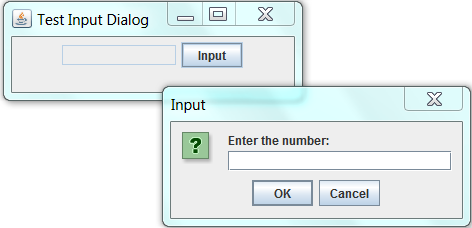
\includegraphics[width=0.8\textwidth]{Input dan GUI Sederhana/InputDialog.png}
    \caption{Contoh dialog input menggunakan JOptionPane}
    \label{fig:joptionpane}
  \end{figure}
  \begin{block}{}
    \textbf{Sumber: }NTU.edu.sg - Java Programming Tutorial
  \end{block}
\end{frame}

% Section 2: BufferedReader vs Scanner
\section{Scanner vs BufferedReader}
\begin{frame}{Perbandingan:  BufferedReader dan Scanner}
    
  \begin{table}
    \footnotesize
    \begin{tabular}{p{0.15\textwidth}|p{0.37\textwidth}|p{0.32\textwidth}}
    \textbf{Aspek} & \textbf{BufferedReader} & \textbf{Scanner} \\
    \hline
    \rowcolor{lightgray}
    Kapasitas Buffer & 8192 karakter (default) & 1024 karakter \\
    \rowcolor{white}
    Tipe Input & Hanya String & Berbagai tipe data (int, double, boolean, dll) \\
    \rowcolor{lightgray}
    Method Input & read(), readLine() & next(), nextInt(), nextDouble(), nextLine(), dll \\
    \rowcolor{white}
    Kecepatan & Lebih cepat untuk teks besar & Lebih lambat \\
    \rowcolor{lightgray}
    Parsing Data & Manual parsing diperlukan & Otomatis parsing ke tipe data \\
    \end{tabular}
    \caption{Perbandingan BufferedReader dan Scanner}
  \end{table}
  
  \begin{block}{}
    \textbf{Sumber: }docs.oracle.com - Oracle Java 25 Documentation
  \end{block}
\end{frame}
\begin{frame}[fragile]{Scanner vs BufferedReader: Input Integer}
  \begin{columns}
    \begin{column}{0.48\textwidth}
      \textbf{Menggunakan\\Scanner}
      \begin{lstlisting}
System.out.println(
    "Masukkan 2 angka:");
Scanner baca = 
    new Scanner(System.in);
int angka1 = baca.nextInt();
int angka2 = baca.nextInt();




      \end{lstlisting}
    \end{column}
    \begin{column}{0.48\textwidth}
      \textbf{Menggunakan BufferedReader}
      \begin{lstlisting}
System.out.println(
    "Masukkan 2 angka:");
BufferedReader baca = 
    new BufferedReader(
    new InputStreamReader(System.in));
int angka1 = Integer.parseInt(
    baca.readLine());
int angka2 = Integer.parseInt(
    baca.readLine());
      \end{lstlisting}
    \end{column}
  \end{columns}
\end{frame}

% Section 3: Implementasi Scanner
\section{Implementasi Scanner}
\begin{frame}[fragile]{Deklarasi dan Penggunaan Scanner}
  \begin{block}{Import dan Deklarasi}
    \begin{lstlisting}
// Import package Scanner
import java.util.Scanner;

public class InputScanner {
    public static void main(String[] args) {
        // Deklarasi Scanner
        Scanner baca = new Scanner(System.in);
    }
}
    \end{lstlisting}
  \end{block}
\end{frame}

\begin{frame}[fragile]{Method-Method Scanner}
  \begin{block}{Method Penting Scanner}
    \begin{lstlisting}
// Membaca berbagai tipe data
String kata = baca.next();        // Satu kata
String kalimat = baca.nextLine(); // Satu kalimat
int angka = baca.nextInt();       // Integer
double pecahan = baca.nextDouble(); // Double
float desimal = baca.nextFloat();  // Float
boolean logika = baca.nextBoolean(); // Boolean
byte nilaiByte = baca.nextByte();  // Byte
short nilaiShort = baca.nextShort(); // Short
long nilaiLong = baca.nextLong();  // Long
    \end{lstlisting}
  \end{block}
\end{frame}

\begin{frame}[fragile]{Contoh Program Scanner}
\begin{lstlisting}
import java.util.Scanner;

public class InputNama {
    public static void main(String[] args) {
        System.out.println("Masukkan nama Anda:");
        Scanner baca = new Scanner(System.in);
        String nama = baca.nextLine();
        System.out.println("Nama anda adalah " + nama);
    }
}
\end{lstlisting}
\end{frame}

% Section 4: Implementasi BufferedReader
\section{Implementasi BufferedReader}
\begin{frame}[fragile]{Deklarasi BufferedReader}
  \begin{block}{Import dan Deklarasi}
    \begin{lstlisting}
// Import package untuk BufferedReader
import java.io.BufferedReader;
import java.io.InputStreamReader;

public class InputBufferedReader {
    public static void main(String[] args) {
        // Deklarasi BufferedReader
        BufferedReader baca = new BufferedReader(
            new InputStreamReader(System.in));
    }
}
    \end{lstlisting}
  \end{block}
\end{frame}

\begin{frame}[fragile]{Penggunaan BufferedReader}
  \begin{block}{Membaca Input dengan BufferedReader}
    \begin{lstlisting}
// Membaca input sebagai String
String kalimat = baca.readLine();

// Membaca tipe data lain (harus di-parse)
int angka = Integer.parseInt(baca.readLine());
double pecahan = Double.parseDouble(baca.readLine());
float desimal = Float.parseFloat(baca.readLine());
long bilanganBesar = Long.parseLong(baca.readLine());
short bilanganKecil = Short.parseShort(baca.readLine());
byte nilaiByte = Byte.parseByte(baca.readLine());
boolean status = Boolean.parseBoolean(baca.readLine());
    \end{lstlisting}
  \end{block}
\end{frame}

\begin{frame}[fragile]{Contoh Program BufferedReader}
\begin{lstlisting}
import java.io.BufferedReader;
import java.io.InputStreamReader;

public class InputBiodataBuffered {
    public static void main(String[] args) {
        BufferedReader baca = new BufferedReader(
            new InputStreamReader(System.in));
        
        System.out.println("Masukkan nama:");
        String nama = baca.readLine(); // Langsung String
        
        System.out.println("Masukkan umur:");
        int umur = Integer.parseInt(baca.readLine()); // Parse ke int
\end{lstlisting}
\end{frame}

\begin{frame}[fragile]{Contoh Program BufferedReader}
\begin{lstlisting}
        System.out.println("Masukkan IPK:");
        double ipk = Double.parseDouble(baca.readLine()); // Parse ke double
        
        System.out.println("Nama: " + nama + 
                         ", Umur: " + umur + 
                         ", IPK: " + ipk);
    }
}
\end{lstlisting}

\begin{block}{Keterangan}
- \texttt{readLine()} selalu mengembalikan \textbf{String}\\
- \texttt{Integer.parseInt()} untuk parsing ke \textbf{int}\\
- \texttt{Double.parseDouble()} untuk parsing ke \textbf{double}
\end{block}
\end{frame}

% Section 5: Parsing Data
\section{Parsing Data}
\begin{frame}[fragile]{Penjelasan Parsing Data}
  \begin{block}{Apa itu Parsing?}
    \textbf{Parsing} = proses mengubah String ke tipe data lain
  \end{block}
\end{frame}

\begin{frame}[fragile]{Scanner: Parsing Otomatis}
  \textbf{Scanner} melakukan parsing otomatis dari input ke tipe data yang diinginkan
  
  \begin{exampleblock}{Contoh Parsing Otomatis}
    \begin{lstlisting}
// Langsung ke tipe data yang diinginkan
int umur = scanner.nextInt();
double ipk = scanner.nextDouble();
boolean status = scanner.nextBoolean();
    \end{lstlisting}
  \end{exampleblock}
\end{frame}

\begin{frame}[fragile]{BufferedReader: Parsing Manual}
  \textbf{BufferedReader} hanya membaca input sebagai String.\\Programmer harus melakukan parsing manual ke tipe data yang diinginkan
  
  \begin{exampleblock}{Contoh Parsing Manual}
    \begin{lstlisting}
// Input selalu sebagai String
String inputNama = bufferedReader.readLine();
String inputUmur = bufferedReader.readLine();
String inputIpk = bufferedReader.readLine();

// Parsing manual diperlukan
String nama = inputNama; // Sudah String
int umur = Integer.parseInt(inputUmur);
double ipk = Double.parseDouble(inputIpk);
boolean aktif = Boolean.parseBoolean(inputAktif);
    \end{lstlisting}
  \end{exampleblock}
\end{frame}

% Section 6: GUI dengan JOptionPane
\section{GUI dengan JOptionPane}
\begin{frame}[fragile]{Pengenalan JOptionPane}
  \begin{block}{Apa itu JOptionPane?}
    \begin{itemize}
      \item \textbf{Fitur} untuk membuat dialog box sederhana
      \item Bagian dari \texttt{javax.swing} (tools untuk GUI)
      \item Mudah digunakan untuk input/output berbasis GUI
      \item Tidak perlu coding kompleks untuk tampilan dialog
    \end{itemize}
  \end{block}
  
  \begin{block}{Cara Menggunakan JOptionPane}
    \begin{lstlisting}
// Tambahkan ini di awal file
import javax.swing.JOptionPane;
    \end{lstlisting}
  \end{block}
\end{frame}

\begin{frame}[fragile]{Method-Method JOptionPane}
  \begin{block}{Method Utama JOptionPane}
    \begin{lstlisting}
// Meminta input dari user
String input = JOptionPane.showInputDialog("Pesan");

// Menampilkan pesan ke user
JOptionPane.showMessageDialog(null, "Pesan");

// Menanyakan konfirmasi (yes/no/cancel)
int pilihan = JOptionPane.showConfirmDialog(null, "Pesan");
    \end{lstlisting}
  \end{block}
\end{frame}

\begin{frame}[fragile]{Contoh Program JOptionPane}
\begin{lstlisting}
import javax.swing.JOptionPane;

public class InputGUI {
    public static void main(String[] args) {
        // Input dari user
        String nama = JOptionPane.showInputDialog(
            "Masukkan nama Anda:");
        
        // Output ke user
        String message = "Nama anda adalah " + nama;
        JOptionPane.showMessageDialog(null, message);
    }
}
\end{lstlisting}
\end{frame}

% Section 7: Contoh Program Kombinasi
\section{Contoh Program Kombinasi}
\begin{frame}[fragile]{Program Input Biodata (Scanner \& JoptionPane)}
\begin{lstlisting}
import java.util.Scanner;
import javax.swing.JOptionPane;

public class BiodataMahasiswa {
    public static void main(String[] args) {
        Scanner baca = new Scanner(System.in);
        
        System.out.println("Masukkan nama:");
        String nama = baca.nextLine();
        
        System.out.println("Masukkan NRP:");
        int nrp = baca.nextInt();
        baca.nextLine(); // membersihkan buffer
\end{lstlisting}
\end{frame}
\begin{frame}[fragile]{Program Input Biodata (Scanner \& JoptionPane)}
\begin{lstlisting}
        System.out.println("Masukkan kota asal:");
        String kota = baca.nextLine();
        
        String output = "Nama: " + nama + 
                       "\nNRP: " + nrp + 
                       "\nKota Asal: " + kota;
        JOptionPane.showMessageDialog(null, output);
    }
}
\end{lstlisting}

\begin{block}{Keterangan}
- Input melalui \textbf{Scanner} (konsol)\\
- Output melalui \textbf{JOptionPane} (GUI)\\
- \texttt{baca.nextLine()} untuk membersihkan buffer setelah \texttt{nextInt()}
\end{block}
\end{frame}
\begin{frame}[fragile]{Program Input Nilai (BufferedReader \& JOptionPane)}
\begin{lstlisting}
import java.io.BufferedReader;
import java.io.InputStreamReader;
import javax.swing.JOptionPane;

public class InputNilaiMahasiswa {
    public static void main(String[] args) {
        BufferedReader baca = new BufferedReader(
            new InputStreamReader(System.in));
        
        System.out.println("Masukkan nama:");
        String nama = baca.readLine();
        
        System.out.println("Masukkan nilai:");
        double nilai = Double.parseDouble(baca.readLine());
        
        // Tentukan grade
        String grade;
\end{lstlisting}
\end{frame}

\begin{frame}[fragile]{Program Input Nilai (BufferedReader \& JOptionPane)}
\begin{lstlisting}
        if (nilai >= 85) grade = "A";
        else if (nilai >= 70) grade = "B";
        else if (nilai >= 60) grade = "C";
        else grade = "D";
        
        String output = "Nama: " + nama + 
                       "\nNilai: " + nilai + 
                       "\nGrade: " + grade;
        JOptionPane.showMessageDialog(null, output);
    }
}
\end{lstlisting}

\begin{block}{Keterangan}
- Input melalui \textbf{BufferedReader} (konsol)\\
- Output melalui \textbf{JOptionPane} (GUI)\\
- Parsing manual: \texttt{Double.parseDouble()}\\
- Logika if-else untuk menentukan grade
\end{block}
\end{frame}

% Section 8: Latihan
\section{Latihan}
\begin{frame}{Latihan 1}
  \begin{block}{Soal 1}
    Buatlah program menggunakan \textbf{Scanner} untuk membaca:
    \begin{itemize}
      \item Nama lengkap
      \item Umur (integer)
      \item IPK (double)
    \end{itemize}
    Cetak hasil input ke layar menggunakan GUI (JOptionPane)
  \end{block}
\end{frame}

\begin{frame}{Latihan 1}
  \begin{block}{Soal 2}
    Buat program menggunakan \textbf{BufferedReader} yang:
    \begin{itemize}
      \item Membaca 2 buah bilangan bulat
      \item Menjumlahkan kedua bilangan
      \item Menampilkan hasilnya di konsol
    \end{itemize}
  \end{block}
\end{frame}

\begin{frame}{Latihan 3}
  \begin{block}{Soal 3}
    Buatlah program menggunakan \textbf{Scanner} yang:
    \begin{itemize}
      \item Meminta input 2 bilangan pecahan (double)
      \item Menjumlahkan, mengurangkan, mengalikan, dan membagi kedua bilangan
      \item Menampilkan semua hasil operasi ke layar
    \end{itemize}
  \end{block}
\end{frame}

% Section 9: Kesimpulan
\section{Kesimpulan}
\begin{frame}{Kesimpulan}
  \begin{alertblock}{Inti Bab 4}
    \begin{itemize}
      \item \textbf{Scanner} dan \textbf{BufferedReader} adalah dua cara utama untuk membaca input dari konsol di Java.
      \item \textbf{Scanner} lebih praktis karena bisa langsung membaca berbagai tipe data.
      \item \textbf{BufferedReader} lebih cepat, tetapi hasil input selalu berupa \texttt{String} sehingga perlu parsing manual.
      \item \textbf{JOptionPane} digunakan jika ingin membuat input dan output berbasis GUI dengan cara yang sederhana.
      \item Pemilihan metode input tergantung kebutuhan, kemudahan, kecepatan, dan tampilan yang diinginkan.
    \end{itemize}
  \end{alertblock}
\end{frame}


% Section 10: Referensi
\section{Referensi}
\begin{frame}{Referensi}
  \begin{block}{Referensi:}
    \begin{itemize}
      \item \textbf{NTU Java GUI Programming}\\
            \url{https://www3.ntu.edu.sg/home/ehchua/programming/java/J4a_GUI_2.html}
      \item \textbf{Oracle Java 25 Documentation}\\
            \url{https://docs.oracle.com/en/java/javase/25/docs/api/index.html}
    \end{itemize}
  \end{block}
\end{frame}

% Penutup
\begin{frame}[standout]
  \Huge \textbf{Terima Kasih} \\[1.5em]
  \Large Pertanyaan dan Diskusi
\end{frame}

\end{document}